\section{System test}
After the Assembling of the PCB and testing the components behave like the expectation, the system test is performed. At first the converter is subjected the open loop test. The reason of this test is to compare the results with the values from the ideal open loop simulation in section \ref{opsimresult}. The second test includes the thermal test. The converter is performed for a longer time. This will be done to identify which parts of the PCB will produce too much heat. The last test is about validating the P\&O MPPT algorithm, if it behaves like same as in the simulation from section \ref{MPPTSimulation}.

\subsection{Open loop test}
For the open loop test the converter is tested one time in buck and boost mode. Both mode will be test at the MPP. So, the constant input voltage for both test is 36.9 V. The environmental condition in these cases is 1000 $W /m^2$ for the irradiance and 25 $\decC$ for the temperature. For both test the current and the voltage ripple are measured to check if they have same value as calculate. Also the steady state of the experimental results are validated with the values from the simulation.

For the buck mode the load is 3 $\Omega$ at the output. With the fix duty cycles $D1 = 0.65$ and  $D2 = 0$ , the output voltage should be 24 V in steady state . The figure shows the transition of the converter in open loop. After special number seconds  the voltages is reaching the steady state. Comparing to figure \ref{} in the simulation section, the ripple are very high Here a sentence about the comparing with the simulation.  In the figure the output voltage is 21.1 V  at steady state less than the expected value, hence there are losses in the system.
The main losses are the dissipation from the component in heat. Also the load is a power resistor and it changes the resistance if it is in operation. So we have not a constant load at the output as in the simulation. Another reason is the dead-time of the MOSFET and therefore the duty cycle is not exactly the same value as in the simulation. From the equation \ref{effiencybuckmode} the efficiency of the system is 87.5$\%$.

\begin{equation}\label{effiencybuckmode}
\eta = \frac{V_{outputexperimantel}}{V_{output simulation}} \cdot 100 = \frac{21.1V}{24V} \cdot 100 = 87.5 \%
\end{equation}
\todo{maybe we dont need here the effiency}
For the boost mode the load is 27 $\Omega$ at the output. With the fix duty cycles $D1 = 1$ and  $D2 = 0.638$ , the output voltage should be 90 V in steady state . The figure shows the transition to reach the steady state. Here a sentence about the comparing with the simulation.  In the figure the output voltage is -- V  at steady state.

The table \ref{tab:ripple} compares the values of the ripples from the experiments with the values from the requirement and from the simulation in section \ref{opsimresult}. So in all three cases the measured ripples from the experiment are higher/lower than the values from the requirement.Here the reason.

\begin{table}[H]
	\centering
	\begin{tabular}{|>{\centering}p{3.5cm}|p{3cm}|p{3cm}|p{3cm}|}
		\hline
		\rowcolor{lightgray} \textbf{} & \textbf{Requirement} & \textbf{Simulation}  & \textbf{Experiment}   \tabularnewline \hline
		$\Delta V_{in}$ & 36.9 mV [0.1\%] & &   \tabularnewline \hline
		$\Delta I_{L}$ & 323 mV [10\%]&  & \tabularnewline \hline
		$\Delta V_{out}$  & 450 mV [0.5\%]  & & \tabularnewline \hline
		
	\end{tabular}
	\caption{Voltage and current ripple.}
	\label{tab:ripple}
\end{table}


\subsection{Thermal test}

For this test, the converter is supplied for 10 minutes (or 600 seconds) a constant input voltage 36.9 V and input current 7 A. Tthe converter is performing in buck mode with the fix duty cycles D1 = 0.8 and D2 = 0 in this test. The temperature of the components coil, heat sink and security diode are measured during the test because they are the critical components. Figure \ref{Testthermal} shows that the diode is produced the most amount of heat.\todo {thats not true. This is only a random sentence.}

\begin{figure}[H]
	\begin{center}
		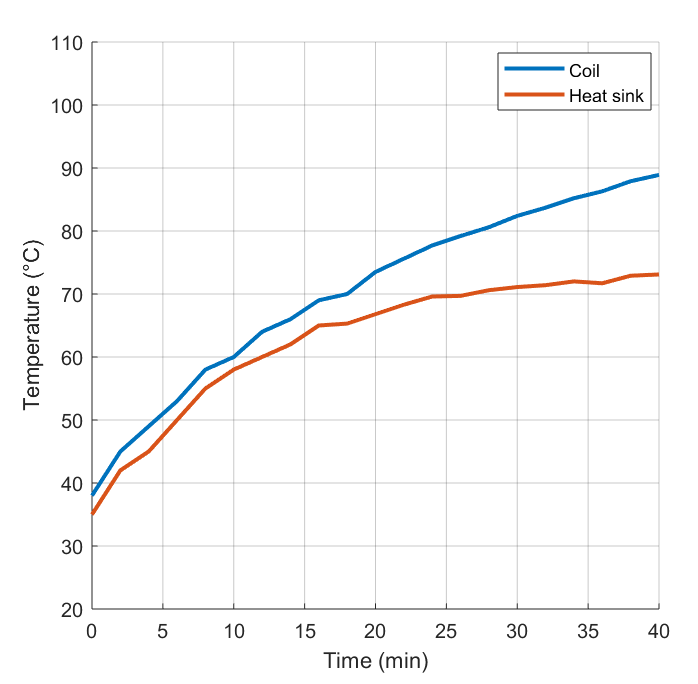
\includegraphics[width=0.65\textwidth]{../Pictures/P1/Test/Thermal_test_with_heat_sink}
		\caption{Thermal test.}
		\label{Testthermal}
	\end{center}	
\end{figure}

\subsection{MPPT test}
The section MPPT test is divided in two parts. One part is that the converter is working with the P\&O to find the MPP .The other part is that during the converter with the P\&O MPPT algorithm is in operation the ambient conditions will change in temperature or irradiance. The tests are compared with the result from section \ref{MPPTSimulation}. The MPPT frequency for all tests is 10 Hz and is ten times smaller as the simulation one. The PV-panel voltage and current is in all figures the input voltage and current from the converter.

In the first part the converter is operated one time in buck and boost mode. For both modes the ambient condition is for the irradiance 1000 $W /m^2$ and for the temperature 25 $\decC$ (as STC ). If the converter is performed in the buck mode, the load is 3 $\Omega$ at the output from the converter. For the boost mode the load is 27 $\Omega$ at the output.

The figure \ref{MPPTtestbuckmode} shows that the converter is finding the MPP. The left graph represents the relationship between the input and output voltage and the current of the converter. At first the input voltage is not reaching the open circuit voltage like in the simulation.  After 6 seconds the P\&O algorithm reachs the MPP. \todo{for the future: compare with the values the simulation with the experiment in one graph. but consider that the simulation should run for 40 seconds to plot both in one graph}

\begin{figure}[H]
	\begin{center}
		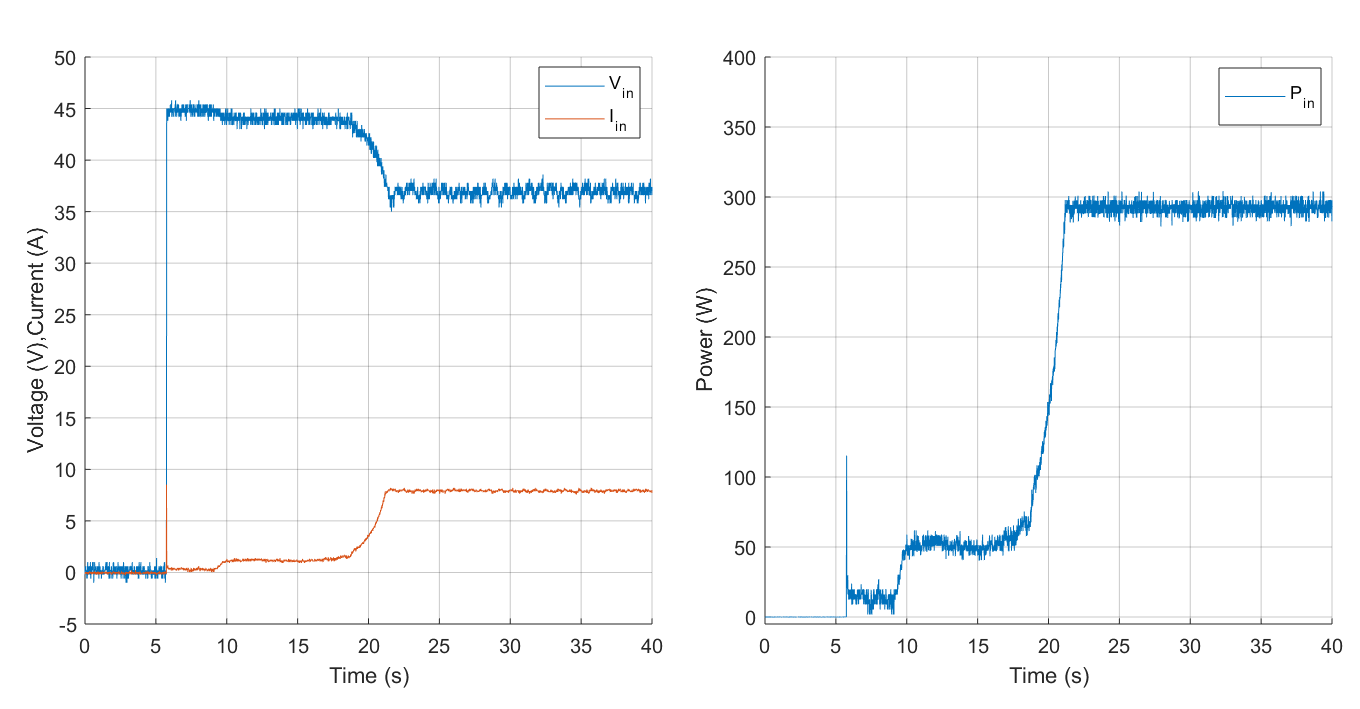
\includegraphics[width=1\textwidth]{../Pictures/P1/Test/Boost_mode_MPPT_Vin_Iin_Pin}
		\caption{MPPT test: converter in boost mode}
		\label{MPPTtestboostmode}
	\end{center}	
\end{figure}



\begin{itemize}
	\item which time is the converter reaching the MPP 
	
	\item what is different as at the simulation
	
	\item at first Iin Vin then P
\end{itemize}





